% Auto-generated by plot_pe_training_comparison.py
% Requires: \usepackage{caption, booktabs, multirow}
% Left table + right figure. In main doc: % Auto-generated by plot_pe_training_comparison.py
% Requires: \usepackage{caption, booktabs, multirow}
% Left table + right figure. In main doc: % Auto-generated by plot_pe_training_comparison.py
% Requires: \usepackage{caption, booktabs, multirow}
% Left table + right figure. In main doc: % Auto-generated by plot_pe_training_comparison.py
% Requires: \usepackage{caption, booktabs, multirow}
% Left table + right figure. In main doc: \input{figures/pe_table_layout.tex}
% or \graphicspath{{figures/}} so the PDF name resolves.
% \\noindent + \\vspace{0pt} fix vertical misalignment of side-by-side [t] minipages.
\begin{figure}[htbp]
\noindent
\begin{minipage}[t]{0.49\textwidth}
\vspace{0pt}
\centering
{\setlength{\heavyrulewidth}{1.2pt}
\begin{tabular}{lcccc}
\toprule
\multirow{2}{*}{Method} & \multicolumn{2}{c}{Last eval} & \multicolumn{2}{c}{Best eval} \\
\cmidrule(lr){2-3}\cmidrule(lr){4-5}
 & avg & var & avg & var \\
\midrule
DSPG & \textbf{5.6612} & \textbf{0.003222} & 5.7315 & \textbf{0.000642} \\
PPO & 5.1279 & 0.131985 & \textbf{5.9101} & 0.066618 \\
SAC & 4.2658 & 0.059560 & 4.7163 & 0.019283 \\
DDPG & 4.5016 & 0.500776 & 5.2248 & 0.220691 \\
\specialrule{.1em}{0pt}{0pt}
VFI & 5.6534 & --- & 5.6534 & --- \\
\bottomrule
\end{tabular}
}
\captionof{table}{Partial-equilibrium methods: ergodic discounted utility (avg and sample variance across random seeds). Bold: best avg per column; best (lowest) var per column.}
\label{tab:pe_ergodic_summary}
\end{minipage}
\hfill
\begin{minipage}[t]{0.49\textwidth}
\vspace{0pt}
\centering
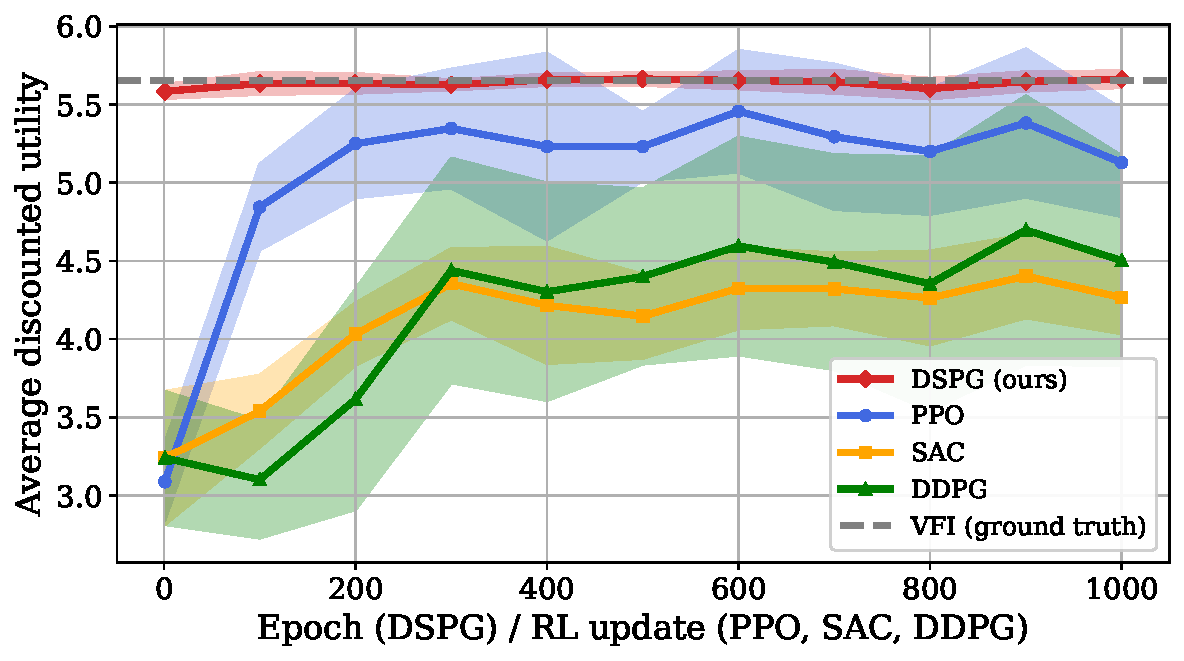
\includegraphics[width=\linewidth]{pe_DSPG_PPO_SAC_DDPG_VFI_training_curves.pdf}
\captionof{figure}{Training curves: DSPG vs PPO vs SAC vs DDPG vs VFI (ergodic discounted utility).}
\label{fig:pe_training_curves}
\end{minipage}
\end{figure}

% or \graphicspath{{figures/}} so the PDF name resolves.
% \\noindent + \\vspace{0pt} fix vertical misalignment of side-by-side [t] minipages.
\begin{figure}[htbp]
\noindent
\begin{minipage}[t]{0.49\textwidth}
\vspace{0pt}
\centering
{\setlength{\heavyrulewidth}{1.2pt}
\begin{tabular}{lcccc}
\toprule
\multirow{2}{*}{Method} & \multicolumn{2}{c}{Last eval} & \multicolumn{2}{c}{Best eval} \\
\cmidrule(lr){2-3}\cmidrule(lr){4-5}
 & avg & var & avg & var \\
\midrule
DSPG & \textbf{5.6612} & \textbf{0.003222} & 5.7315 & \textbf{0.000642} \\
PPO & 5.1279 & 0.131985 & \textbf{5.9101} & 0.066618 \\
SAC & 4.2658 & 0.059560 & 4.7163 & 0.019283 \\
DDPG & 4.5016 & 0.500776 & 5.2248 & 0.220691 \\
\specialrule{.1em}{0pt}{0pt}
VFI & 5.6534 & --- & 5.6534 & --- \\
\bottomrule
\end{tabular}
}
\captionof{table}{Partial-equilibrium methods: ergodic discounted utility (avg and sample variance across random seeds). Bold: best avg per column; best (lowest) var per column.}
\label{tab:pe_ergodic_summary}
\end{minipage}
\hfill
\begin{minipage}[t]{0.49\textwidth}
\vspace{0pt}
\centering
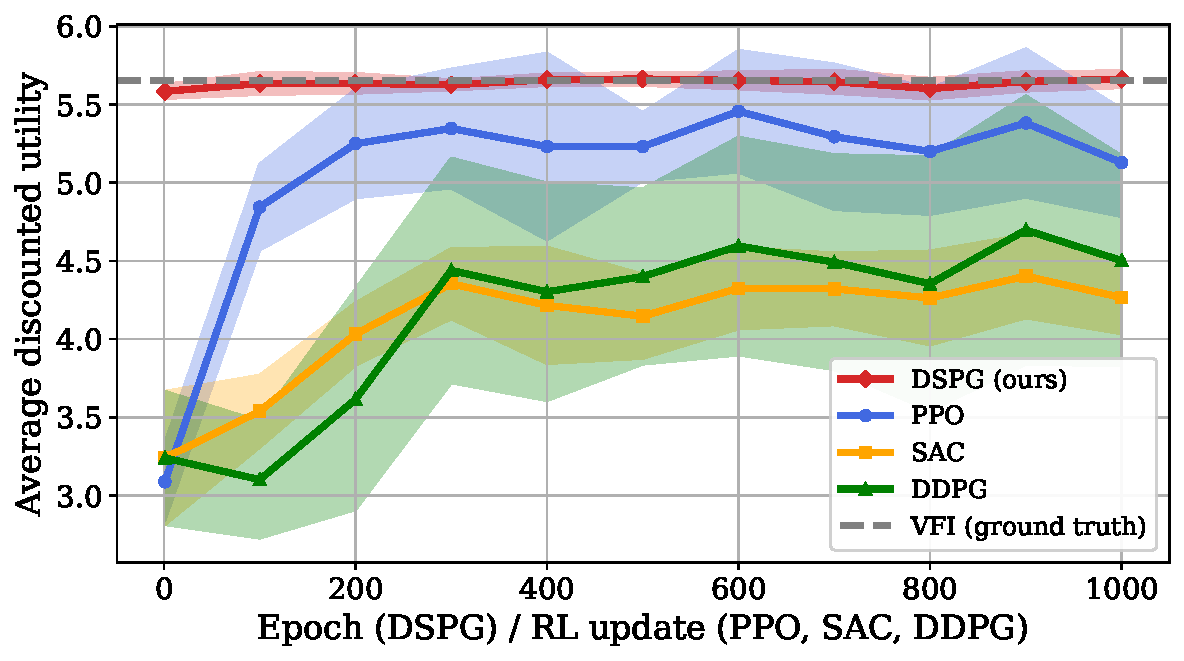
\includegraphics[width=\linewidth]{pe_DSPG_PPO_SAC_DDPG_VFI_training_curves.pdf}
\captionof{figure}{Training curves: DSPG vs PPO vs SAC vs DDPG vs VFI (ergodic discounted utility).}
\label{fig:pe_training_curves}
\end{minipage}
\end{figure}

% or \graphicspath{{figures/}} so the PDF name resolves.
% \\noindent + \\vspace{0pt} fix vertical misalignment of side-by-side [t] minipages.
\begin{figure}[htbp]
\noindent
\begin{minipage}[t]{0.49\textwidth}
\vspace{0pt}
\centering
{\setlength{\heavyrulewidth}{1.2pt}
\begin{tabular}{lcccc}
\toprule
\multirow{2}{*}{Method} & \multicolumn{2}{c}{Last eval} & \multicolumn{2}{c}{Best eval} \\
\cmidrule(lr){2-3}\cmidrule(lr){4-5}
 & avg & var & avg & var \\
\midrule
DSPG & \textbf{5.6612} & \textbf{0.003222} & 5.7315 & \textbf{0.000642} \\
PPO & 5.1279 & 0.131985 & \textbf{5.9101} & 0.066618 \\
SAC & 4.2658 & 0.059560 & 4.7163 & 0.019283 \\
DDPG & 4.5016 & 0.500776 & 5.2248 & 0.220691 \\
\specialrule{.1em}{0pt}{0pt}
VFI & 5.6534 & --- & 5.6534 & --- \\
\bottomrule
\end{tabular}
}
\captionof{table}{Partial-equilibrium methods: ergodic discounted utility (avg and sample variance across random seeds). Bold: best avg per column; best (lowest) var per column.}
\label{tab:pe_ergodic_summary}
\end{minipage}
\hfill
\begin{minipage}[t]{0.49\textwidth}
\vspace{0pt}
\centering
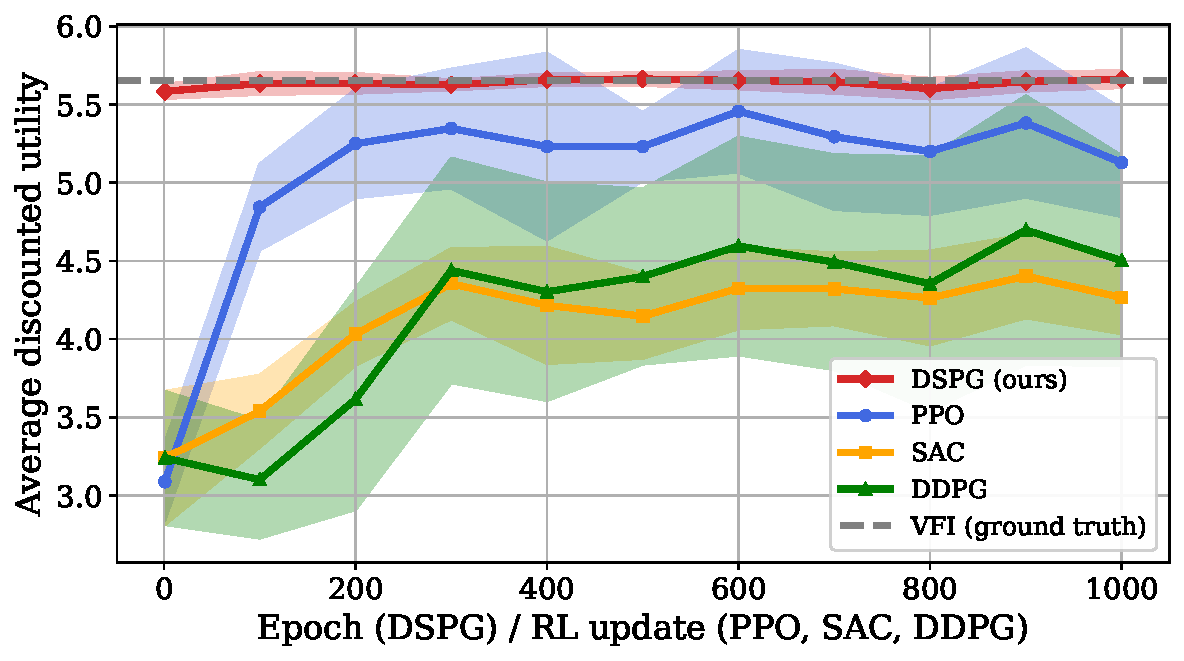
\includegraphics[width=\linewidth]{pe_DSPG_PPO_SAC_DDPG_VFI_training_curves.pdf}
\captionof{figure}{Training curves: DSPG vs PPO vs SAC vs DDPG vs VFI (ergodic discounted utility).}
\label{fig:pe_training_curves}
\end{minipage}
\end{figure}

% or \graphicspath{{figures/}} so the PDF name resolves.
% \\noindent + \\vspace{0pt} fix vertical misalignment of side-by-side [t] minipages.
\begin{figure}[htbp]
\noindent
\begin{minipage}[t]{0.49\textwidth}
\vspace{0pt}
\centering
{\setlength{\heavyrulewidth}{1.2pt}
\begin{tabular}{lcccc}
\toprule
\multirow{2}{*}{Method} & \multicolumn{2}{c}{Last eval} & \multicolumn{2}{c}{Best eval} \\
\cmidrule(lr){2-3}\cmidrule(lr){4-5}
 & avg & var & avg & var \\
\midrule
DSPG & \textbf{5.6612} & \textbf{0.003222} & 5.7315 & \textbf{0.000642} \\
PPO & 5.1279 & 0.131985 & \textbf{5.9101} & 0.066618 \\
SAC & 4.2658 & 0.059560 & 4.7163 & 0.019283 \\
DDPG & 4.5016 & 0.500776 & 5.2248 & 0.220691 \\
\specialrule{.1em}{0pt}{0pt}
VFI & 5.6534 & --- & 5.6534 & --- \\
\bottomrule
\end{tabular}
}
\captionof{table}{Partial-equilibrium methods: ergodic discounted utility (avg and sample variance across random seeds). Bold: best avg per column; best (lowest) var per column.}
\label{tab:pe_ergodic_summary}
\end{minipage}
\hfill
\begin{minipage}[t]{0.49\textwidth}
\vspace{0pt}
\centering
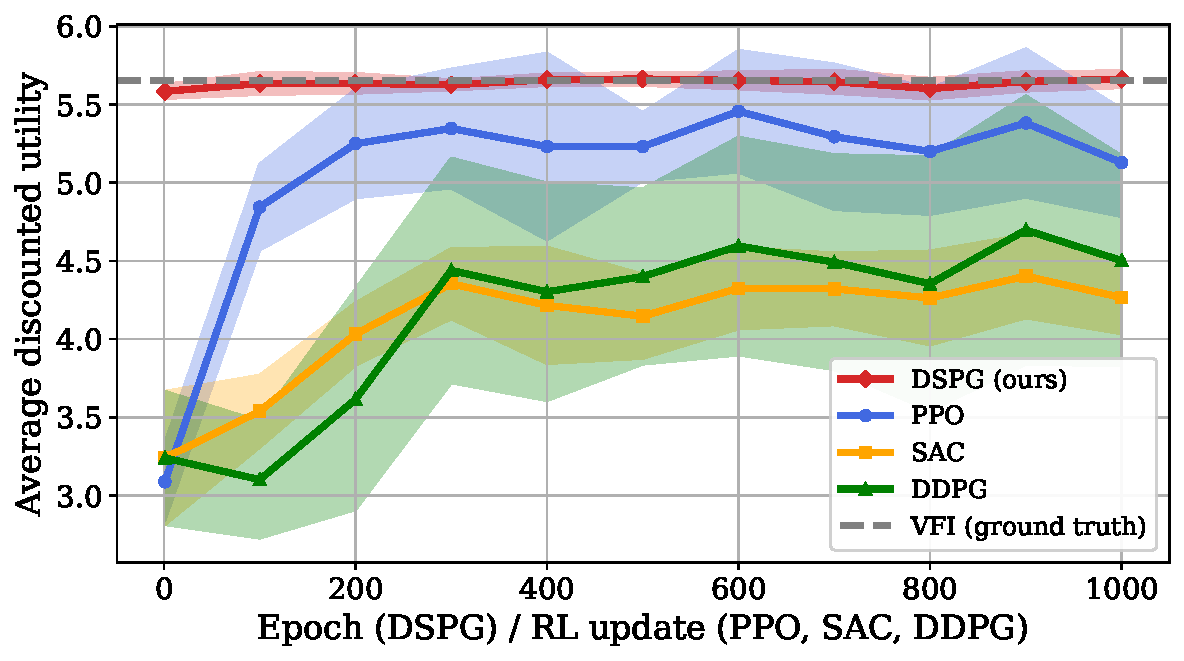
\includegraphics[width=\linewidth]{pe_DSPG_PPO_SAC_DDPG_VFI_training_curves.pdf}
\captionof{figure}{Training curves: DSPG vs PPO vs SAC vs DDPG vs VFI (ergodic discounted utility).}
\label{fig:pe_training_curves}
\end{minipage}
\end{figure}
